Si bien representar características es común en todo proyecto de ML, hacerlo con texto suele ser más complejo que con otros tipos de datos. Consideremos ejemplos como imágenes: almacenamos imágenes como matrices de píxeles, cada uno representando la intensidad de un píxel en la imagen. Con videos, cada cuadro se convierte en una matriz. En cuanto al habla, registramos la amplitud de una onda sonora en intervalos de tiempo fijos. Sin embargo, representar matemáticamente texto después de haberlo dividido en alguna unidad léxica para luego deducir el significado de cada unidad, comprender la estructura gramatical, entender el contexto en el que aparece y finalmente gracias a estos datos discernir la semántica, no es tan fácil. Esta sección  se sumerge en múltiples esquemas para abordar esta complejidad, desde métodos simples hasta las últimas técnicas para representar texto, un desafío que ha sido un foco activo de investigación en las últimas décadas.

Los enfoques tomados para generar todo tipo de representaciones de texto que se detallaran a continuación, pueden ser: 

\begin{itemize}

	\item Similitud Distribucional : El significado de una palabra se extrae del contexto en el que aparece, no sólo del significado literal.

	\item Hipótesis Distribucional: Plantea que palabras en contextos similares tienen significados similares. La similitud entre palabras se basa en sus contextos de aparición.
	
	\item Representación Distribucional: Se basa en esquemas que utilizan vectores de alta dimensión para representar palabras, basados en una matriz de co-ocurrencia, misma que captura la co-ocurrencia de palabras y contextos.
	
	\item Representación Distribuida: Una versión más compacta y densa en vectores que la representación distribucional, para superar la ineficiencia computacional de los vectores altamente dimensionales.

	\item Incrustación: Es un mapeo entre el espacio vectorial de la representación distributiva y la representación distribuida para un conjunto de palabras.
	
	\item Semántica Vectorial: Métodos de PLN que buscan aprender representaciones de palabras basadas en propiedades distribucionales en grandes corpus.
\end{itemize}

En el campo del PNL, transformar texto en una forma numérica se llama representación de texto. A continuación se explorarán los distintos métodos para convertir texto en vectores numéricos, todos los que se encuentran clasificados como modelos espaciales vectoriales como one-hot, bag of words, bag of n-grams y TF-IDF  caen dentro del concepto de representación distribucional.

\begin{itemize}
\item Modelos espaciales vectoriales


Los modelos vectoriales espaciales son técnicas que representan las palabras como vectores en un espacio dimensional. Estos modelos tienen como objetivo capturar la semántica de las palabras al asignarles vectores en un espacio matemático, donde la proximidad entre los vectores refleja la similitud semántica entre las palabras. Un modelo de espacio vectorial  es un modelo algebraico simple, en su representación simple son vectores identificadores como un índice de números en un vocabulario de algún documento, párrafo o libro de texto. El modelo más común para medir esta similitud, es la similitud del coseno, ver ecuacion \ref{eq:e21}. Por ejemplo las frases: ``El cielo es azul'' y ``El sol es amarillo'', se pueden representar cada una como un vector numérico. Para calcular la similitud entre estos vectores, se puede utilizar  el coseno del ángulo entre ellos. Si estos vectores se alinean perfectamente, el coseno del ángulo es 1, lo que indica una similitud máxima. Si están en direcciones opuestas, el coseno es -1, lo que significa una similitud mínima.
\begin{equation} \label{eq:e21} 
	similarity = cos(\theta) = \frac{\mathbf{A} \cdot \mathbf{B}}{\left \|  \mathbf{A} \right \|_2\cdot \left \|  \mathbf{B} \right \|_2}=\frac{\displaystyle\sum_{i=1}^{n}A_iB_i}{\sqrt{\displaystyle\sum_{i=1}^{n}A_i^2}\sqrt{\displaystyle\sum_{i=1}^{n}B_i^2}}
\end{equation}


$A = $  Algun vector.\\
$B = $  Algun vector.\\
$\mathbf{A} \cdot \mathbf{B} =$ Es el producto punto entre los vectores $A$ y $B$.\\
$\left \|  \mathbf{A} \right \|_2\cdot \left \|  \mathbf{B} \right \|_2 = $ Indica la norma euclidiana o la norma $L_2$. \\
$L_2$  de un vector = Se calcula sumando el cuadrado de cada componente del vector y luego tomando la raíz cuadrada del resultado. Que es equivalente a: 
$\left \|  \mathbf{A} \right \|_2 = \sqrt{A_1^2 + A_2^2 + \cdots + A_n^2} $.\\


La calidad de los vectores depende de cómo capturan las propiedades lingüísticas del texto. Diferentes enfoques, como el conteo de palabras o modelos de lenguaje pre-entrenados (word embeddings), producen representaciones de texto en forma de vectores con diferentes niveles de fidelidad y utilidad.

\begin{itemize}

	\item ONE HOT ENCODING: En One-Hot Encoding, cada palabra se representa mediante un vector binario donde todas las posiciones son cero excepto una, que corresponde al índice de la palabra en un vocabulario. Si hay un total de N palabras en el vocabulario, cada palabra se representa como un vector de longitud N con un único ``1'' en la posición que indica su índice en el vocabulario y ``0'' en todas las demás posiciones. Por ejemplo, si se tiene un vocabulario con las palabras: ``perro'', ``gato'', ``pájaro'' y ``muerde'', la representación One-Hot de cada una sería:
\begin{Center}
	perro → [1, 0, 0,0]\\
	gato → [0, 1, 0,0]\\
	pájaro → [0, 0, 1,0]\\
	muerde → [0, 0, 0, 1]\\
	
\end{Center}

Donde:

La oración ``perro muerde gato'' sería representada como: [   [1, 0 ,0 , 0]   [0, 0, 0, 1]   [0, 1, 0, 0]  ]


Este tipo de representación textual  es intuitiva y fácil de implementar pero, presenta limitaciones significativas. La relación directa entre el tamaño del vector one-hot y el tamaño del vocabulario provoca representaciones dispersas donde la mayoría de las entradas son ceros, lo que resulta en ineficiencia computacional y riesgo de sobreajuste. Además, esta representación no ofrece una longitud fija para el texto y trata las palabras como entidades aisladas, careciendo de la capacidad para capturar relaciones semánticas entre ellas. El desafío de manejar palabras fuera del vocabulario (Out Of Vocabulary), no se puede abordar directamente con esta representación, se requiere la expansión y reentrenamiento del modelo para incluir nuevas palabras.

	\item BAG OF WORDS: El modelo Bag of Words (BoW) es una técnica básica  para representar texto numéricamente. Primero  se construye un vocabulario a partir del corpus de documentos. El vocabulario se compone de todas las palabras únicas presentes en el corpus, y cada palabra se la enumera de manera única. Luego, se representa cada documento como un vector numérico. Para ello, se cuenta la frecuencia de cada palabra del vocabulario en cada documento. Por ejemplo: 
Dada las oraciones: \textit{``El gato está en la casa gato''} y \textit{``El perro está afuera''}

Se construye el diccionario: {El=1, gato=2, está=3, en=4, la=5, casa=6, perro=7, afuera=8}. Los IDs serán enteros únicos entre $\left | \text{V} \right |$, Donde $\left | \text{V} \right |$ representa el tamaño del vocabulario.

Se realiza la representación BoW:
\begin{center}
	\begin{tabular}{c c c c c c c c c c}
		& El & gato & está & en & la & casa & perro & afuera &  \\
		Frase 1: & 1 & 2 & 1 & 1 & 1 & 1 & 0 & 0 & ←Conteo frase 1\\
		Frase 2: & 1 & 0 & 1 & 0 & 0 & 0 & 1 & 1 & ←Conteo frase 2\\
		
	\end{tabular}
\end{center}


El enfoque de BoW trata el texto como una colección de palabras sin considerar el orden ni el contexto en el que aparecen. Supone que el contenido de un texto asociado a una categoría específica en un conjunto de datos está representado por un conjunto único de palabras. Si dos fragmentos de texto comparten la mayoría de sus palabras, se asume que pertenecen a la misma categoría o grupo, por esta razón se puede inferir la categoría o clase a la que ese texto puede pertenecer. Es importante resaltar que el enfoque BoW simplifica el texto a su esencia más básica: las palabras y su frecuencia, sin tomar en cuenta su secuencia o estructura gramatical.

	\item BAG OF N-GRAMS.- Es una técnica utilizada que extiende el concepto de Bag of Words (BoW) al considerar no solo palabras individuales, sino también secuencias contiguas de palabras llamadas n-gramas.``Capta cierta información de contexto y orden de palabras. Por tanto, el espacio vectorial resultante es capaz de capturar alguna similitud semántica. Los documentos que tienen los mismos n-gramas tendrán sus vectores más cerca entre sí en el espacio euclidiano en comparación con documentos con n-gramas completamente diferentes.''\cite[p. 90]{vajjala2020practical}. Un n-grama es una secuencia continua de ``n'' elementos, que pueden ser caracteres, palabras o algún tipo de token, a medida que n aumente, la dimensionalidad aumentará igual rápidamente. Por ejemplo:

Dadas las oraciones: ``El gato está durmiendo'' y ``El perro está comiendo''

Una representación bigrama de palabras es equivalente a:
[ ``El gato'', ``gato esta'', ``está durmiendo'', ``El perro'', ``perro esta'', ``está comiendo'' ]

La representación BoN constara de un vector de seis dimensiones para cada documento: ``El gato está durmiendo'' → [1,1,1,0,0,0], ``El perro está comiendo'' → [0,0,0,1,1,1 ].


Es importante recordar que al igual que Bag of Words, Bag of N-Grams (BoN) no ofrece una solución directa al problema de OOV (Out Of Vocabulary), es decir, no tiene un mecanismo incorporado para tratar con palabras que no estaban presentes durante el entrenamiento del modelo.


	\item TF-IDF.- A diferencia de las anteriores técnicas de representación de texto, Frecuencia de término-Frecuencia inversa de documentos (Term Frequency-Inverse Document Frequency) es una técnica que evalúa la importancia de una palabra en un documento dentro de un corpus o conjunto de documentos. Su formula general se divide en dos componentes que se explicaran detalladamente. Ver ecuación \ref{eq:e22}

\begin{equation} \label{eq:e22}
	\textrm{TF-IDF} = \textrm{TF} \times \textrm{IDF}
\end{equation}

TF (Frecuencia del término) mide la frecuencia con la que una palabra específica aparece en un documento en relación con el total de palabras en ese documento. Básicamente, es la cantidad de veces que una palabra aparece, dividida por el total de palabras en el documento como se muestra en la ecuacion \ref{eq:e23}. Si una palabra aparece muchas veces en un documento específico, y no aparece en los demás documentos, entonces se considera que la palabra es importante para ese documento específico.

\begin{equation} \label{eq:e23}
	\textrm{TF}(t,d)=\frac{(\textrm{Number of occurrences of term }t\textrm{ in document }d)}{(\textrm{Total number of terms in the document } d)}
\end{equation}

IDF (Frecuencia inversa de documentos) mide la importancia de una palabra a través de todo el conjunto de documentos. Esta métrica reduce el peso de palabras comunes que aparecen en muchos documentos y aumenta el peso de palabras raras que podrían ser más significativas para un documento específico. Es decir, si se considera que una palabra es importante para un documento, pero esta aparece constantemente en los demás documentos entonces disminuye su importancia. Se calcula tomando el logaritmo del inverso de la frecuencia de documentos que contienen el término, y se suma uno para evitar la división por cero si el término no está presente en el corpus.

\begin{equation} \label{eq:e24}
	\textrm{IDF}(t)=\frac{(\textrm{Total number of documents in the corpus})}{(\textrm{Number of documents with term } t \textrm{ in them})}
\end{equation}

Esta técnica de representación se aplica para cada palabra en cada documento y se  pueden usar los vectores obtenidos para calcular la similitud entre dos textos, usando alguna medida de similitud como la distancia euclidiana o la similitud del coseno.


\end{itemize}

\item Representaciones distribuidas

Las representaciones distribuidas de texto buscan capturar el significado de palabras, oraciones o frases considerando su proximidad textual, en un espacio vectorial. Estas representaciones, conocidas como embeddings, abordan los desafíos de dimensionalidad y contexto crucial durante el entrenamiento. Para lograrlo, emplean arquitecturas de redes neuronales que generan representaciones de baja dimensión y alta densidad para palabras y textos.

\begin{itemize}

	\item Word embeddings: Las incrustaciones de palabras (word embeddings) son representaciones vectoriales de palabras en un espacio dimensional, donde cada palabra se asigna a un vector denso. Estos vectores son diseñados de manera que palabras con significados similares están cercanas entre sí en este espacio vectorial, además sus representaciones vectoriales de texto tienen dimensiones bajas y densas en comparación con representaciones one-hot encoding, lo que permite una manipulación más eficiente. Los modelos  más populares pueden ser: Word2Vec, GloVe y FastText, uno de los mayores representantes de los modelos embeddings es Word2Vec, que en si mismo es un conjunto de modelos que fueron fundamentales en el campo del Procesamiento del Lenguaje Natural. Desarrollado por un equipo de investigadores de Google, liderado por Tomás Mikolov, en 2013, fue un avance crucial en la generación de representaciones vectoriales de palabras, basadas en modelos de redes neuronales, cuya idea central era capturar y representar la semántica de las palabras a través de sus contextos en un corpus de texto \cite{mikolov2013efficient}. 
	
	\item Hiperparametros de embeddings: Algunos hiperparámetros comunes al trabajar con embeddings en modelos como Word2vec, GloVe, fastText o incluso en modelos más avanzados incluyen:  La dimensión del embedding, la cual  determina la longitud de los vectores; la ventana de contexto, controla cuántas palabras vecinas se van a considerar y el tamaño del vocabulario, ya que algunos modelos de embeddings tienen un límite en el tamaño del vocabulario a usar. Ajustar estos y otros  hiperparámetros correctamente puede influir significativamente en la calidad y el rendimiento de los embeddings resultantes.``El ajuste de hiperparámetros juega un papel clave: cualquier método funcionará mal si se utilizan los hiperparámetros incorrectos'' \cite[p. 339]{eisenstein2018natural}.
	
	\item Word2Vec.- El modelo Word2Vec se destaca por su capacidad para generar incrustaciones vectoriales significativas y densas para palabras, lo que permite representar el significado semántico de las palabras en un espacio vectorial de dimensiones bajas (vectores de dimensiones 50-500 en vez de varios miles). Su eficiencia para la representación de palabras fue tal, que se observaron habilidades para resolver analogías y capturar relaciones de significado entre palabras como:  
	\begin{Center}
			$Rey - Hombre + Mujer \approx  Reina$.
	\end{Center}

	
Word2vec es un conjunto redes neuronales poco profundas que utilizan la similitud distributiva e hipótesis distributiva para aprender  el significado de las palabras ``El modelo Word2vec perfecciona los valores en $v_w$ al predecir $v_{w'}$, dados los vectores para las demás palabras en el contexto C.'' \cite[p. 95]{vajjala2020practical} .

Word2Vec funciona utilizando dos arquitecturas principales: Continuous Bag of Words (Cbow) y Skip-gram.

\begin{figure}
	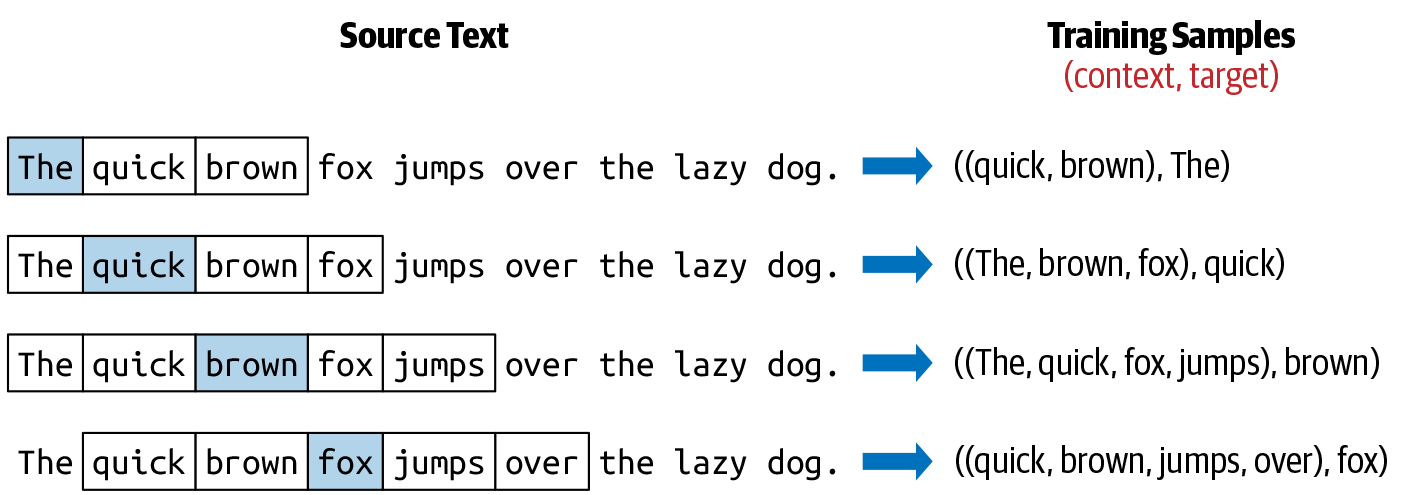
\includegraphics[width=0.65\textwidth]{capitulo3/figuras/nlp3.png}
	\caption{Preparando un conjunto de datos por CBOW}
	\floatfoot{Fuente: Practical natural language processing: A comprehensive guide to building real-world NLP systems \cite[p. 99]{vajjala2020practical}}
	\label{fig:nlp3}
\end{figure}

Cbow: Predice la palabra objetivo basándose en un contexto de palabras adyacentes, tomará cada palabra del corpus como palabra objetivo e intentará predecir la palabra objetivo a partir de sus palabras de contexto correspondientes. Por ejemplo, teniendo un tamaño de contexto dos (k=2), el  tamaño de la ventana deslizante será igual a 2k +1 donde uno representará  a la ventana central. Ver Figura \ref{fig:nlp3}



\begin{figure}[h!]
	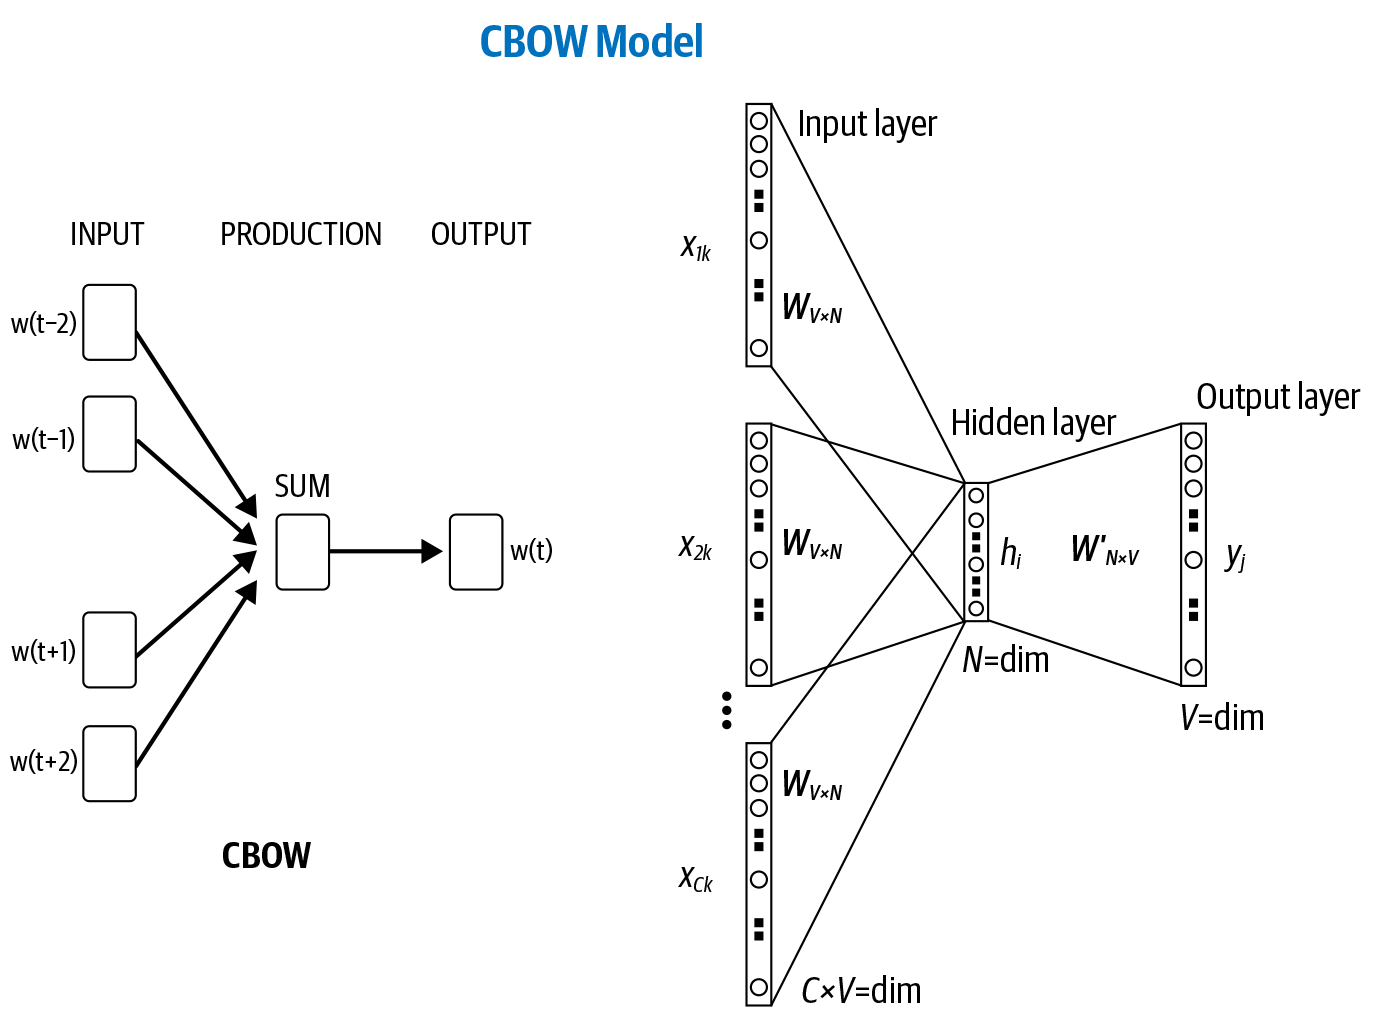
\includegraphics[width=0.65\textwidth]{capitulo3/figuras/nlp4.png}
	\caption{Modelo CBOW}
	\floatfoot{Fuente: Practical natural language processing: A comprehensive guide to building real-world NLP systems \cite[p. 100]{vajjala2020practical}}
	\label{fig:nlp4}
\end{figure}

El modelo Cbow utiliza una red neuronal poco profunda para aprender incrustaciones vectoriales de palabras. Esta red tiene una capa oculta y su objetivo es aprender una matriz de incrustación de palabras (definida como $E_{ \left | \textrm{V}  \right |\: \textrm{x} \: \textrm{d}}$,  donde $\left | \textrm{V}  \right | = $ tamaño del vocabulario, d= dimensión de incrustación)  a partir de un vocabulario (v)  dado inicialmente  \ref{fig:nlp4}. La matriz de incrustación se inicia de forma aleatoria. Posteriormente  la red selecciona vectores de las palabras del contexto de la matriz y los combina para generar un vector (d), que luego se multiplica con otra matriz ${E}'_{ \textrm{d} \: \textrm{x}  \:\left | \textrm{V}  \right | }$ en la siguiente capa. Esto da como resultado un vector de una dimensión por el tamaño del vocabulario ( $1 \times \left | \textrm{V}  \right |$) que funge como entrada para una función softmax para obtener la distribución de probabilidad en el espacio de vocabulario. Al final del entrenamiento, la matriz de incrustación $E$ y $E'$ obtenida se actualizan después de comparar la distribución aprendida con la etiqueta (palabra objetivo) mediante retropropagación.

\begin{figure}[h!]
	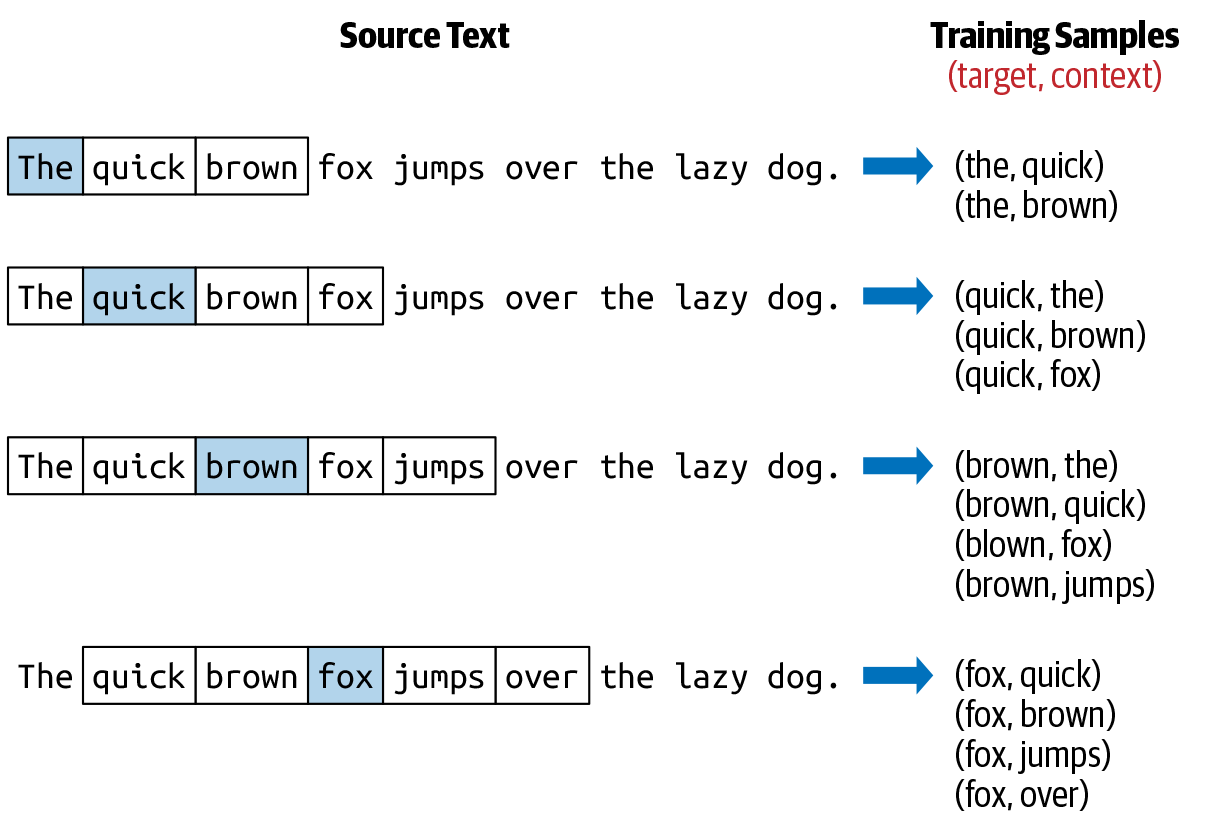
\includegraphics[width=0.65\textwidth]{capitulo3/figuras/nlp5.png}
	\caption{Preparando un conjunto de datos por SkipGram}
	\floatfoot{Fuente: Practical natural language processing: A comprehensive guide to building real-world NLP systems \cite[p. 101]{vajjala2020practical}}
	\label{fig:nlp5}
\end{figure}

Skip-gram: Predice las palabras del contexto a partir de la palabra central. Toma una palabra de entrada y predice las palabras que podrían aparecer en su contexto.``El conjunto de datos para entrenar un SkipGram se prepara de la siguiente manera: ejecutamos una ventana deslizante de tamaño 2k+1 sobre el corpus de texto para obtener el conjunto de 2k+1 palabras que están bajo consideración. La palabra central en la ventana es la X, y las k palabras a cada lado de la palabra central son Y'' \cite[p. 101]{vajjala2020practical}. Al igual que el modelo cbow, k representara el número de palabras, pero en este caso serán las que se deben predecir ver Figura \ref{fig:nlp5}



\begin{figure}
	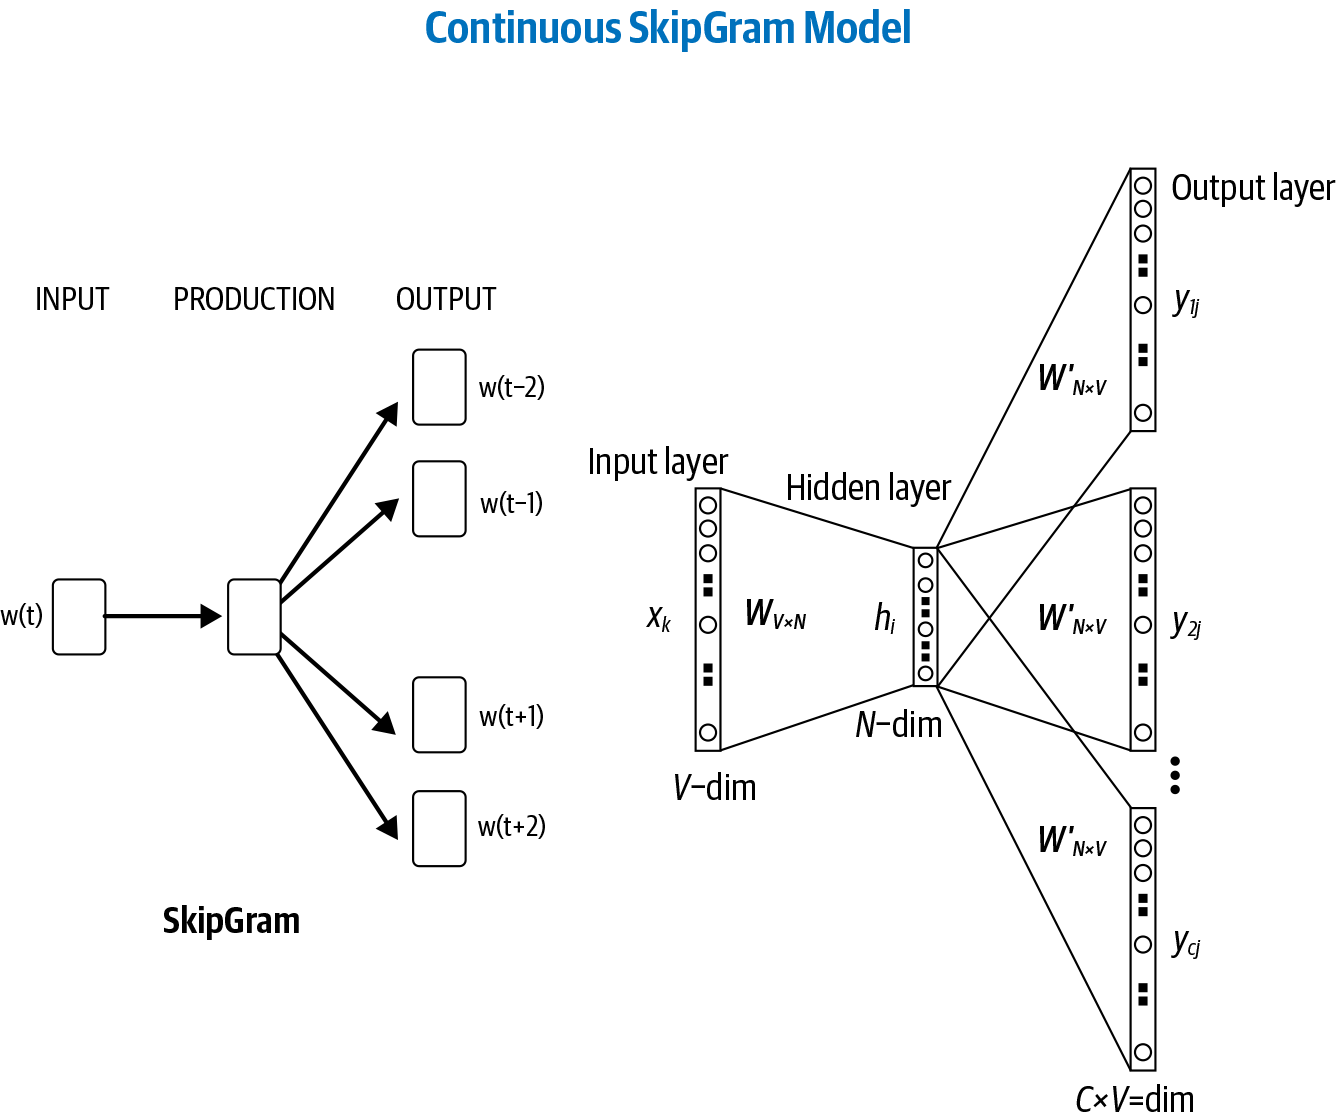
\includegraphics[width=0.65\textwidth]{capitulo3/figuras/nlp6.png}
	\caption{Modelo SkipGram}
	\floatfoot{Fuente: Practical natural language processing: A comprehensive guide to building real-world NLP systems \cite[p. 102]{vajjala2020practical}}
	\label{fig:nlp6}
\end{figure}

En el modelo SkipGram, se emplea una red similar a la usada en CBOW. En la capa de entrada, se toma el índice de la palabra objetivo para acceder a su vector correspondiente en la matriz de incrustación $E_{ \left | \textrm{V}  \right |\: \textrm{x} \: \textrm{d}}$,  donde $\left | \textrm{V}  \right | = $  , estos vectores se combinan y forman un nuevo vector que se multiplica por otra matriz ${E}'_{ \textrm{d} \: \textrm{x}  \:\left | \textrm{V}  \right | }$  para obtener un vector unidimensional de probabilidad en el espacio del vocabulario. La comparación entre esta distribución y la etiqueta se utiliza para actualizar las matrices de incrustación a través de la retropropagación. Al finalizar el entrenamiento, la matriz de incrustación obtenida (denotada como $E_{ \left | \textrm{V}  \right |\: \textrm{x} \: \textrm{d}}$) representara las palabras del vocabulario en vectores de baja dimensión.Ver Figura \ref{fig:nlp6}

	\item Word embeddings pre entrenados:  Son representaciones vectoriales de palabras generadas mediante modelos de lenguaje que han sido entrenados previamente con grandes cantidades de texto. Los embeddings pre entrenados más populares como wor2vec, glove y fastext que ya se mencionaron están disponibles para varias dimensiones como d = 25, 50, 100, 200, 300, 600. De igual forma, en muchas ocasiones, los investigadores comparten embeddings de palabras ya entrenados para ser utilizados libremente en proyectos académicos o comerciales. Cuando se opta por utilizar embeddings previamente entrenados, se tiene dos enfoques principales:
	
Estático: Implica emplear los embeddings tal como están, sin modificarlos. Esto es ideal si los embeddings se ajustan bien al problema y ofrecen buenos resultados.

Actualizado: Se basa en utilizar los embeddings pre entrenados para inicializar el modelo, pero se permite que se actualicen durante el entrenamiento. Esta opción puede ser beneficiosa si se busca integrar y mejorar el modelo en una tarea específica.

Si en estos modelos pre-entrenados no existieran representaciones vectoriales de palabras importantes para la tarea en cuestión, dependiendo de la librería en uso, se pueden reentrenar. 

Para decidir si reentrenar modelos previamente entrenados, una buena regla general es calcular la superposición de vocabulario. Si la superposición entre el vocabulario de nuestro dominio personalizado y el de las incrustaciones de palabras previamente entrenadas es superior al 80\%, las incrustaciones de palabras pre-entrenadas tienden a dar buenos resultados en la clasificación de texto.``Si la superposición entre el vocabulario del corpus y el vocabulario incorporado es inferior al 80\%, es poco probable que veamos un buen desempeño de nuestro modelo de PNL.''\cite[p. 104]{vajjala2020practical}.

	\item Oov y embeddings.- Abordar el problema de las palabras fuera del vocabulario en los modelos de embeddings es todo un desafío, ya que  las palabras fuera del vocabulario no tienen representaciones predefinidas, lo que dificulta su procesamiento y comprensión. Si se quiere rehusar embeddings pre entrenados para saltarse la difícil tarea de entrenar un embedding que requiere de miles y miles de datos para obtener una representación más o menos buena se debe considerar que las representaciones que se encuentren son suficientes y se adaptan al problema, o qué nuevas palabras deben añadirse. Para incorporar palabras nuevas a modelos que ya han sido entrenados, hay algunas estrategias que se pueden utilizar como:

El entrenamiento incremental: implica volver a ejecutar el algoritmo de entrenamiento con el corpus actualizado, que contiene las nuevas palabras. Esto puede ser costoso computacionalmente, en especial si el corpus es grande. 

Inicialización de vectores: Se pueden agregar palabras nuevas asignándoles vectores aleatorios o utilizando algún otro método de inicialización específico.``Una forma de lidiar con el problema OOV para incrustaciones de palabras es crear vectores que se inicializan aleatoriamente, donde cada componente está entre –0,25 y +0,25, y continuar usando estos vectores en toda la aplicación''\cite[p. 105]{vajjala2020practical}.

Sub-palabras: Modelos como FastText abordan el problema de OOV representando las palabras a través de sus constituyentes de caracteres, es decir, descomponiendo las palabras en n-gramas de caracteres (secuencias de caracteres de longitud n. En lugar de solo aprender incrustaciones de palabras completas, también aprende incrustaciones de n-gramas de caracteres. La representación de una palabra se construye agregando las incrustaciones de sus n-gramas de caracteres constituyentes.

Textos Completos:  Otro enfoque para lidiar con el problema OOV, es Doc2Vec. Es una técnica de aprendizaje no supervisado que genera representaciones vectoriales densas para documentos, lo que permite medir la similitud y realizar operaciones semánticas en documentos completos. ``es similar a Word2vec en cuanto a su arquitectura general, excepto que, además de los vectores de palabras, también aprende un ``vector de párrafo'' que representa el texto completo (es decir, con palabras en contexto).''\cite[p.106]{vajjala2020practical}. El vector de párrafo representa un texto completo (un párrafo, una oración o incluso un documento entero). 

Las redes neuronales superficiales utilizadas para aprender las incrustaciones de Doc2vec son parecidas a CBOW y SkipGram de Word2vec, el primer modelo se denomina memoria distribuida (DM) donde se integra tanto la información del contexto de palabras como la representación del documento completo para predecir la palabra objetivo. Esto permite que el modelo capture no solo el significado de las palabras individuales en un contexto, sino también la esencia general del documento en el que aparecen esas palabras. El segundo modelo se denomina bolsa de palabras distribuida (DBOW) este modelo omite la predicción de palabras y se centra únicamente en predecir el siguiente documento basándose solo en el vector de documento.
	
	\item Consideraciones.- A continuación se detallaran consideraciones importantes que tomar respecto al uso de embeddings pre entrenados:\\
Sesgo.-  Las representaciones de texto, como embeddings o vectores que capturan el significado de las palabras o textos, están influenciadas por los datos con los que se entrenan. Estos sesgos pueden tener impactos significativos en el rendimiento de los modelos que dependen de estas representaciones.\\

Exigencia computacional.- Los embeddings pre entrenados suelen ser archivos grandes, a menudo varios gigabytes. Este tamaño puede causar dificultades en el rendimiento si no se aborda adecuadamente. Por ejemplo, el modelo Word2vec requiere aproximadamente 4,5 GB de memoria RAM, lo que puede ser un desafío en ciertos escenarios.
\\
Representar necesidades.- Existen necesidades lingüísticas y de aplicación que van más allá de lo que las técnicas de embeddings pueden capturar actualmente. Por ejemplo, la detección de sarcasmo es una tarea que requiere matices y sutilezas que aún no son bien representadas o entendidas completamente mediante técnicas de embeddings.\\

Estado del arte.- La representación neuronal del texto es un área en constante evolución en el campo del procesamiento del lenguaje natural (PNL), con avances rápidos en el estado del arte. Aunque nuevos modelos suelen generar entusiasmo, es importante considerar aspectos prácticos, usar modelos nuevos no siempre será la mejor opción, es importante considerar que también se pueden tener buenos resultados con modelos de embeddings básicos, que además no requieren de mucha capacidad computacional. 

\end{itemize}
\end{itemize}



